\chapter{Entwurf}
\label{ch:3}

\section{Detailentwurf: Klassen}
\label{sec:3.1}

\subsection{Statik}
\begin{figure}[!htb]
\centering
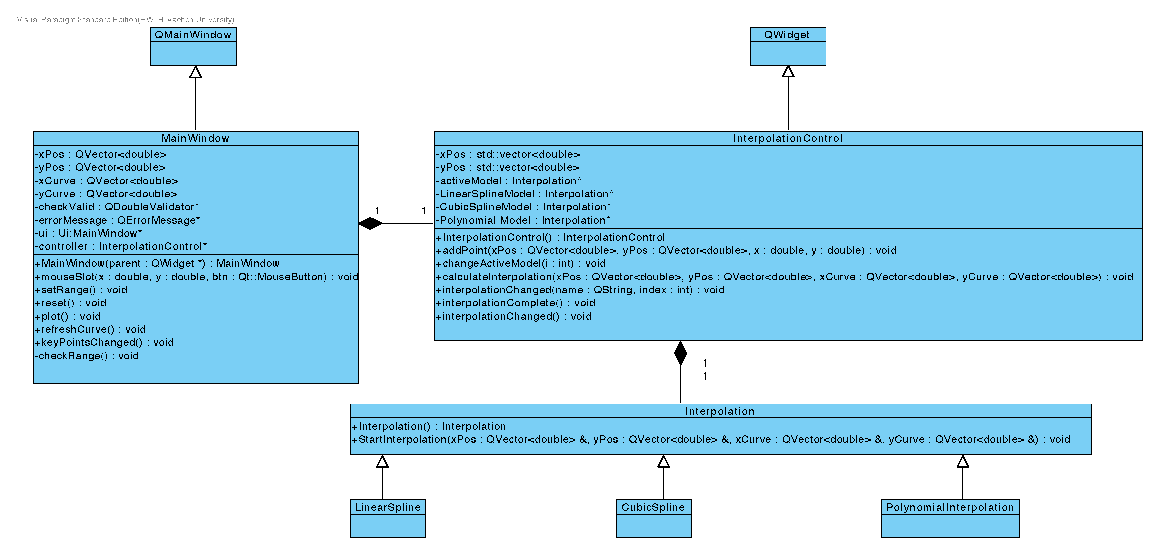
\includegraphics[width=\textwidth]{figures/klassendiagramm.eps}
\caption{Klassendiagramm}
\label{fig:Klassendiagramm}
\end{figure}

\subsection{Dynamik}

\begin{figure}
\centering
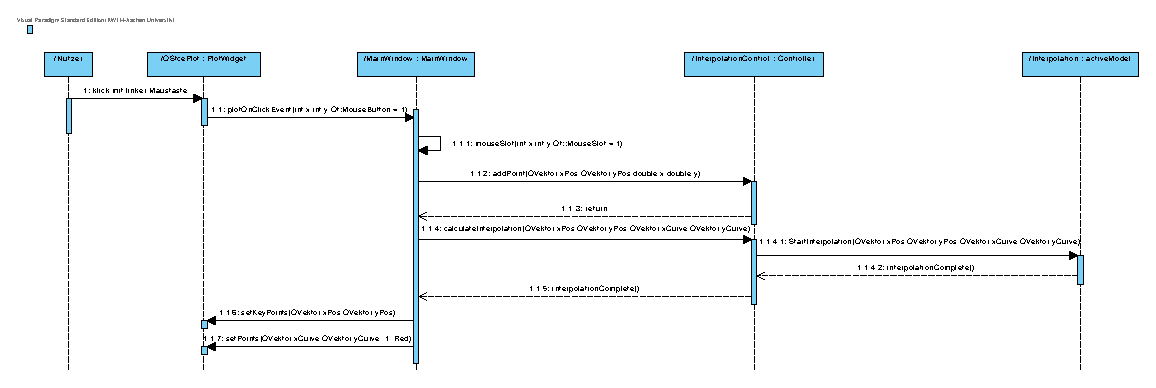
\includegraphics[width=\textwidth]{figures/sequenzdiagramme/mausklick_links_auf_zeichenflaeche.eps}
\caption{Sequenzdiagramm: Stuetzstelle hinzufuegen}
\end{figure}

\begin{figure}
\centering
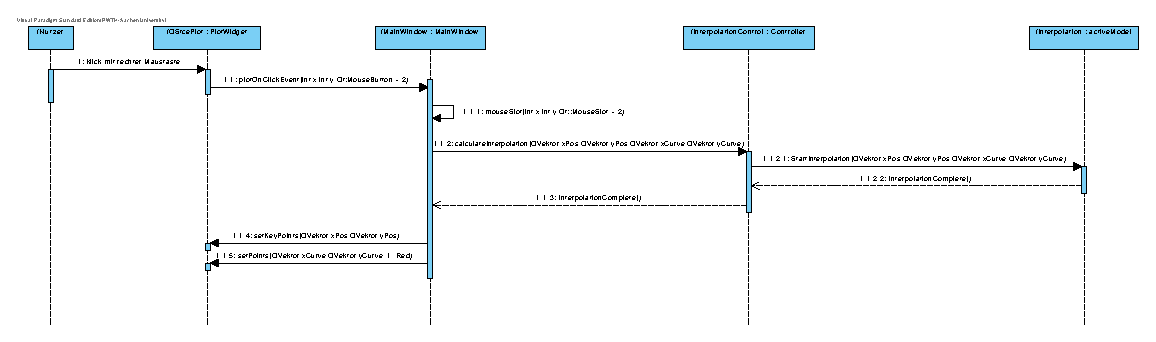
\includegraphics[width=\textwidth]{figures/sequenzdiagramme/mausklick_rechts_auf_zeichenflaeche.eps}
\caption{Sequenzdiagramm: Stuetzstelle loeschen}
\end{figure}

\begin{figure}
\centering
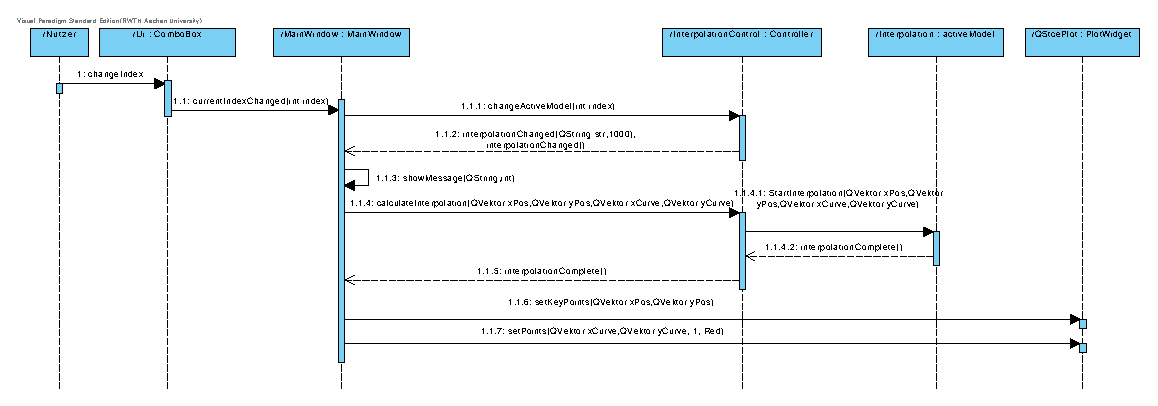
\includegraphics[width=\textwidth]{figures/sequenzdiagramme/interpolation_aendern.eps}
\caption{Sequenzdiagramm: Interpolationsart aendern}
\end{figure}

\begin{figure}
\centering
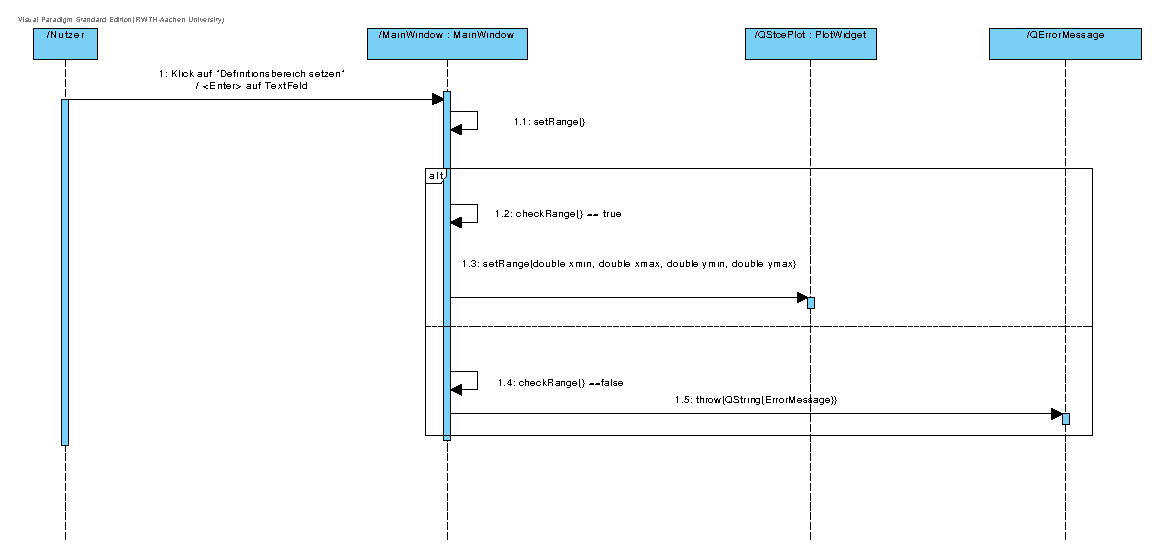
\includegraphics[width=\textwidth]{figures/sequenzdiagramme/definitionsbereich_aendern.eps}
\caption{Sequenzdiagramm: Definitionsbereich aendern}
\end{figure}

\begin{figure}
\centering
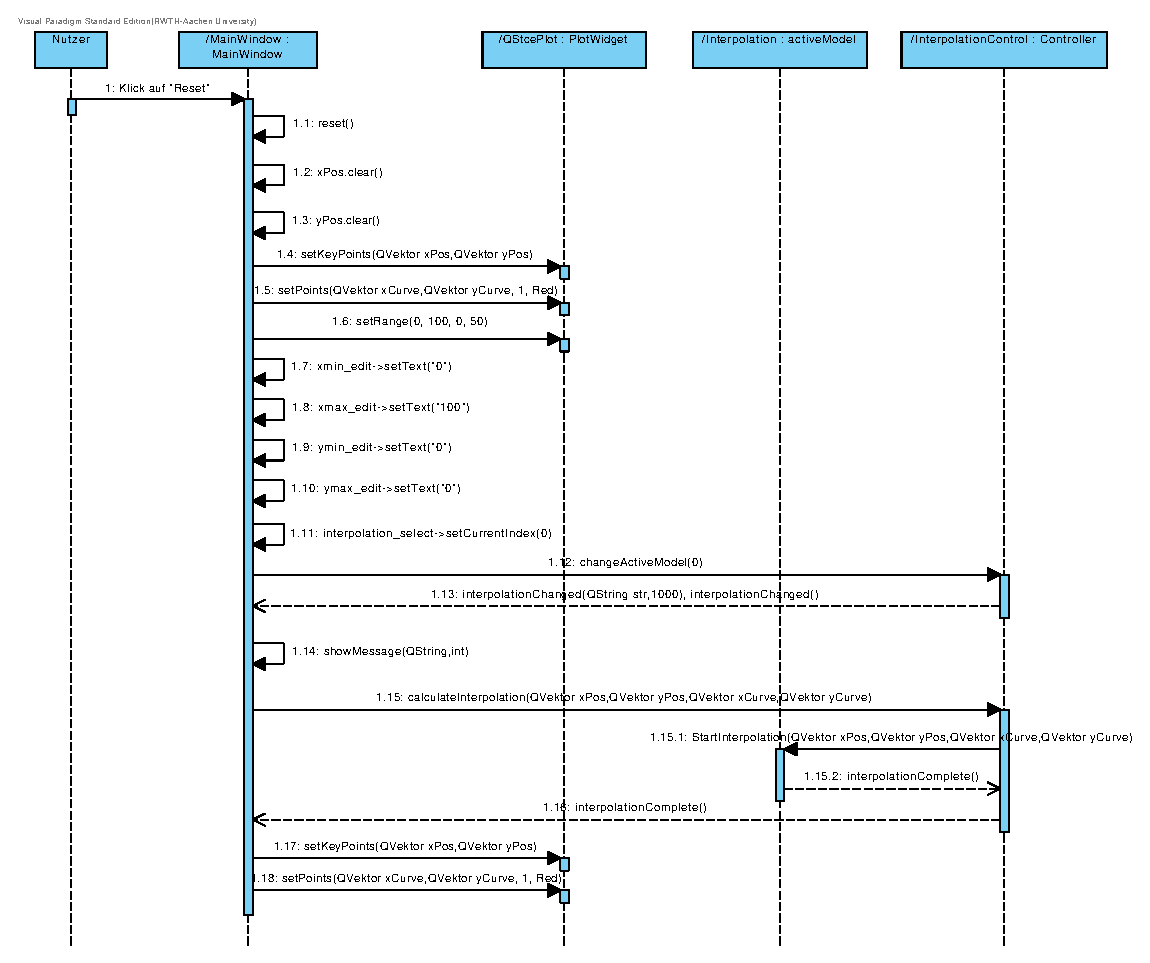
\includegraphics[width=\textwidth]{figures/sequenzdiagramme/Reset.eps}
\caption{Sequenzdiagramm: Reset}
\end{figure}

\begin{figure}
\centering
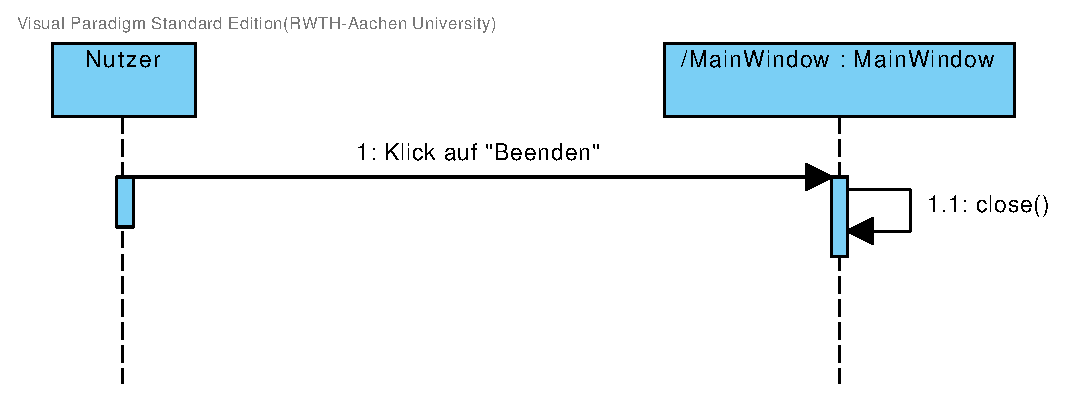
\includegraphics[width=\textwidth]{figures/sequenzdiagramme/Beenden.eps}
\caption{Sequenzdiagramm: Beenden}
\end{figure}